% A physical local attacker is what is traditionally considered when developing TEEs~\cite{costan2016intel,keystone}. With such an attacker only the processor package is trusted, alongside with some low-level software, called security monitor in Keystone and $\mu$Code on Intel SGX. This software is crucial as it incorporates the TEE functionality into RISC-V or Intel processors respectively. In addition, we also trust the peripheral package since a rogue peripheral obviously breaks any secrecy and isolation requirement. We assume the user to be cooperating and interested in getting a correct measurement from the peripheral. So active conspicuous attacks are out of scope.  If, however, the physical world is completely under control of the attacker, then the attacker can change some properties of the physical world such as the temperature or GPS data. Obviously this will lead to a maliciously modified sensor reading and can result in malfunction. However, this attack vector is considered out-of-scope because it usually presents a major hurdle for primitive adversaries (i.e., users). Nevertheless, a sophisticated attacker can take advantage of this and cause tampered sensor readings. Note that this only concerns measurements of the physical world and external accelerators are not affected by this. By trusting the package, we assume that the local attacker can not physically tamper with the processor or the peripherals. However, all connections between the processor and peripherals are fair game and can be fully controlled by an attacker. E.g., on a commercially available desktop platform, the processor package and peripheral ICs (USB, PCI Express) are trusted. However, we also assume that the attacker can also plug her own compromised peripherals into the platform. 

% \subsection{Addressing Local Physical Attacker}


%  \begin{figure}[tbp]
%   \centering
%   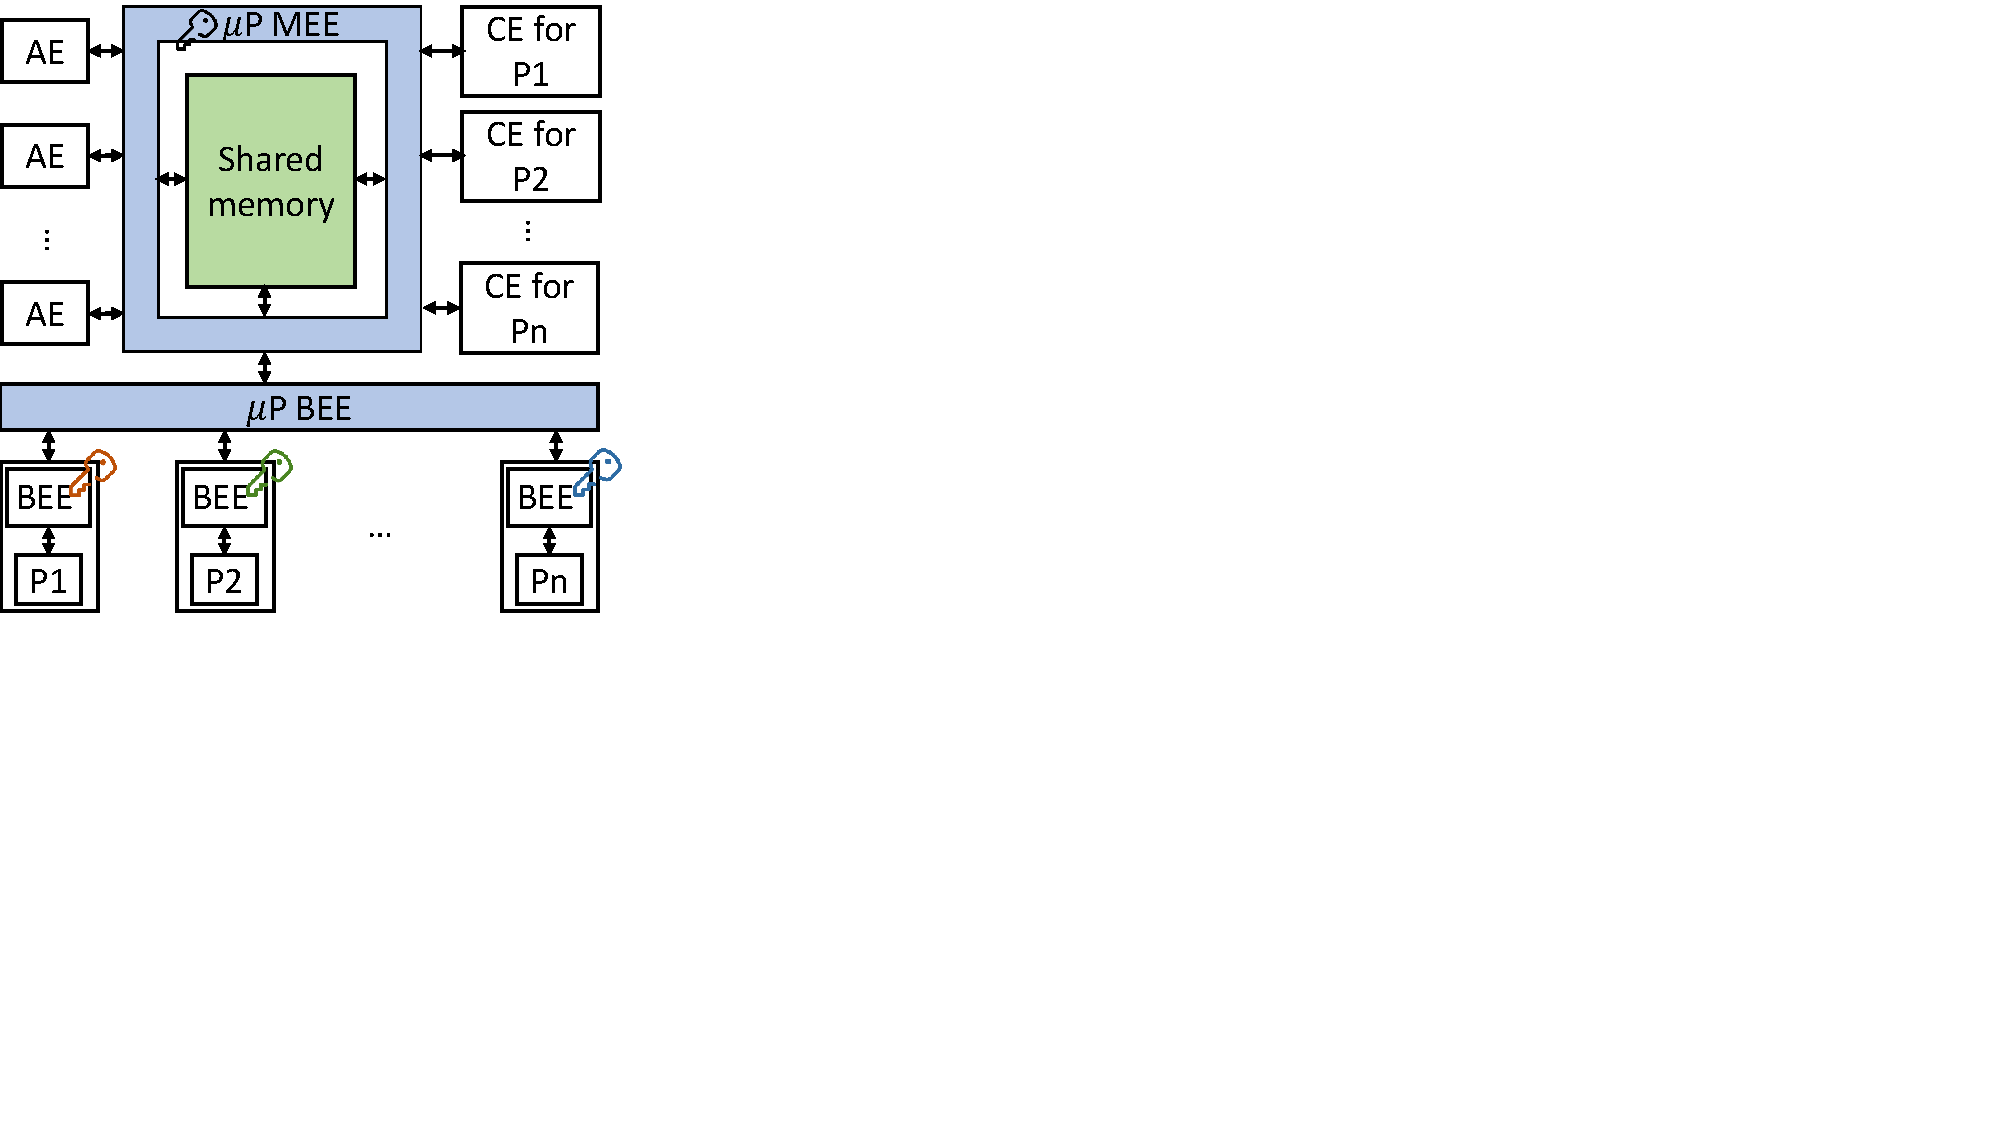
\includegraphics[trim={0 8.5cm 23cm 0}, clip, width=0.7\linewidth]{memoryEnc.pdf}
%   \caption{Different cryptographic engines in relation to different components of \name. AE, CE and MEE stands for application enclave, controller enclave and memory encryption engine respectively.}
%   \label{fig:encEngine}
%  \end{figure}

% \subsubsection{Cryptographic Engines and Key Management}

%  \name relies on memory encryption engine (MEE) and bus encryption engine (BEE) to protect from a local physical attacker. Figure~\ref{fig:encEngine} shows these cryptographic engine in context to various \name programming model components.

% \myparagraph{Memory encryption engine (MEE)} All the enclaves that are running on the CPU cores (\app and \ce) and all the shared memory regions are encrypted by the MEE. Due to this, the attacker who has physical access to the memory module can not observe or manipulate the shared memory contains. As the only the CPU cores access these memories, only one key is sufficient to encrypt and preserve the integrity of the data in all the memory regions. Note that the CPU keeps the integrity tree of all of the shared memory and enclave memory regions.

% \myparagraph{Bus encryption engine (BEE)} MEE is not sufficient in the communication between the CPU core enclaves and peripheral enclaves. In MEE, as mentioned before, the CPU keeps the integrity tree. This is sufficient as only the CPU cores write and read to and from the DRAM. However, when we consider the communication between the CPU core enclaves and the peripheral enclaves, the integrity tree only at the CPU core does not ensure the integrity of the data coming from the peripherals. Due to this, we leverage the bus encryption engine that is present both in the CPU and the peripherals. During the initial attestation process, the CPU and the peripherals derive the session key that is used as the BEE keys. Note that every peripheral derives its own key to communicate with the CPU. This was, an attacker-controlled peripheral can not observe or modify the data on the bus coming from another peripheral.  


% \begin{figure}[t]
%   \centering
%   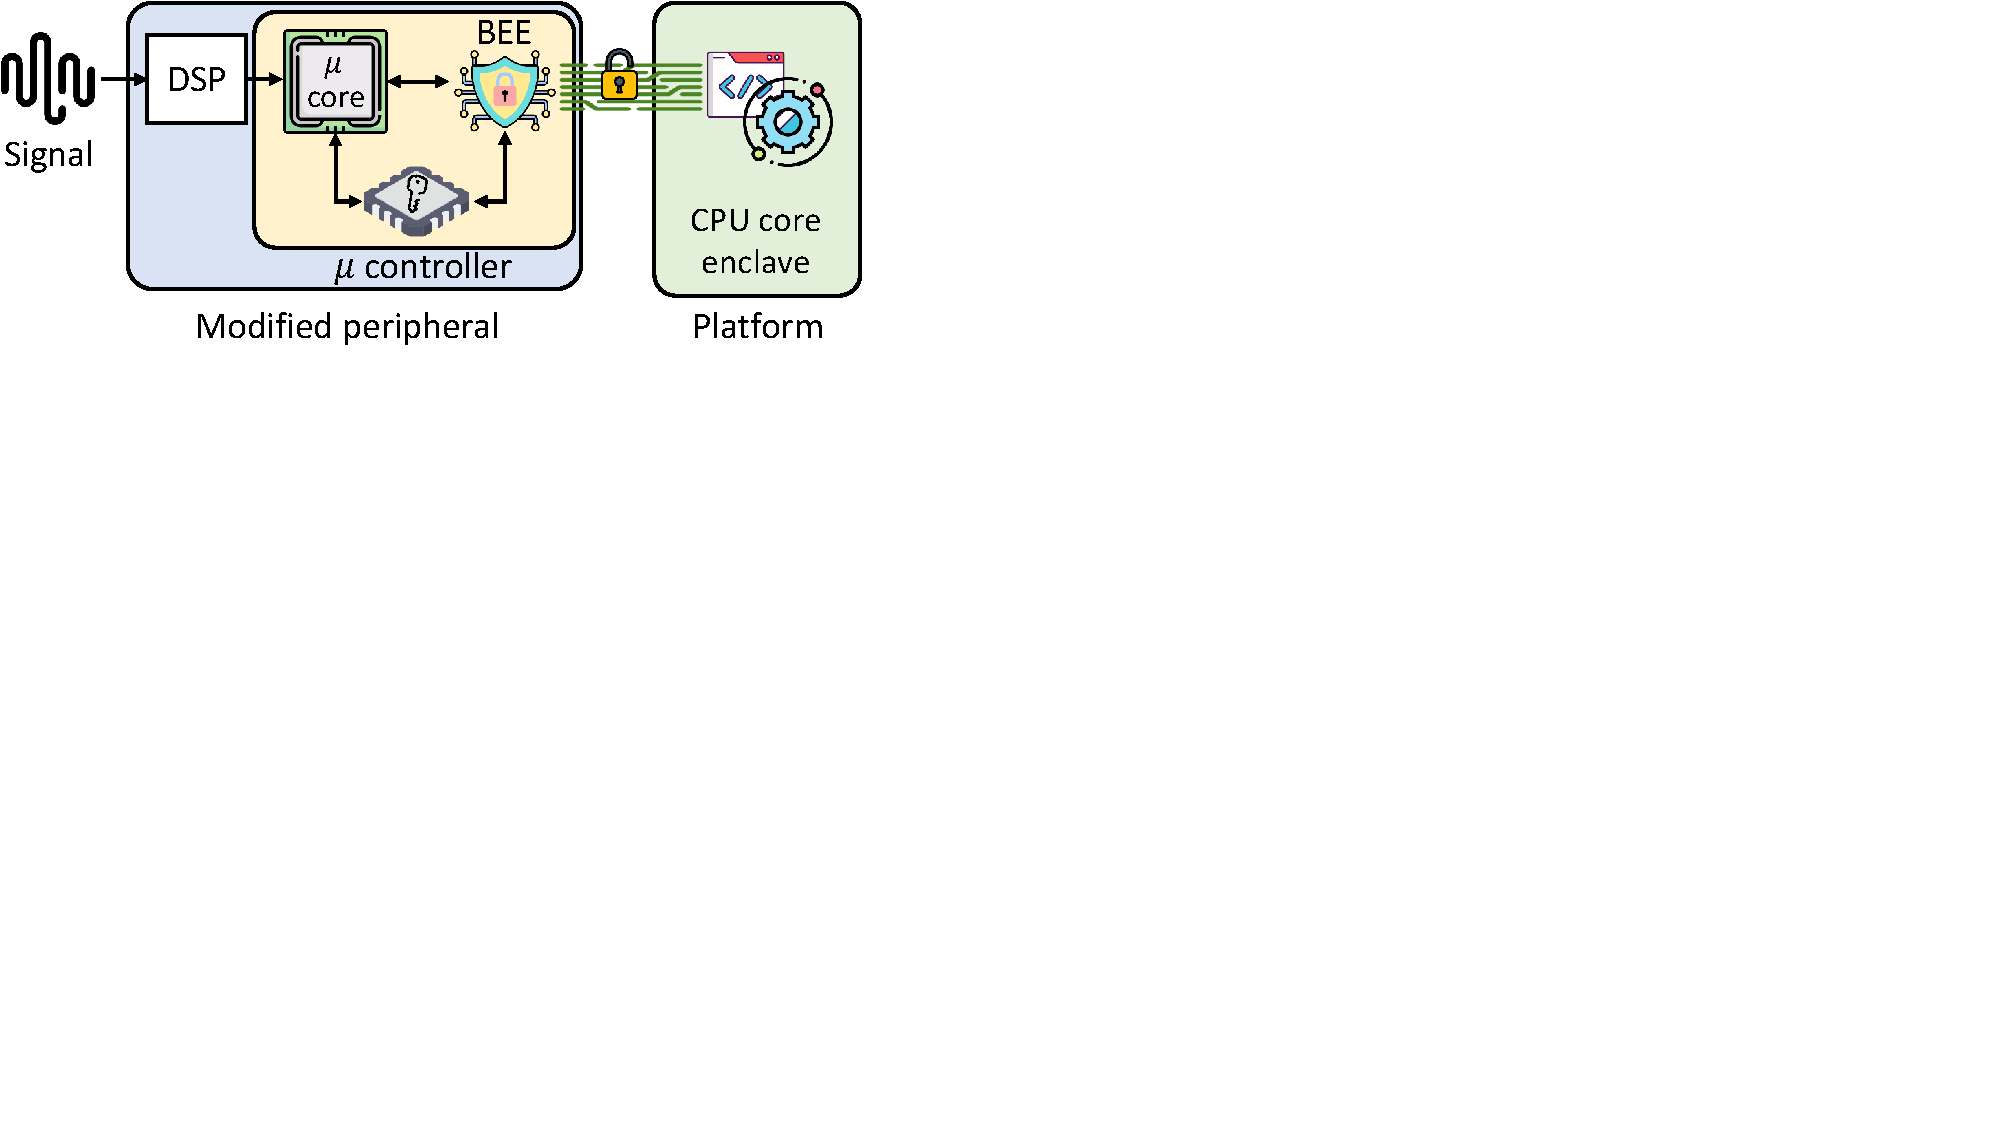
\includegraphics[trim={0 13cm 18cm 0}, clip, width=\linewidth]{peripheral.pdf}
%   \caption{An example peripheral with modifications for \name{} that adds the bus encryption engine (BEE) and a keystorage to communicate with the CPU.}
%   \label{fig:sensor}
% \end{figure}



% \subsubsection{Modified Peripherals}


% The peripherals themselves require some changes in order to be part of platform-wide enclaves. Here we describe one potential peripheral configuration and what modifications are necessary. The modifications to the peripherals enhance their functionality by remote attestation, and bus encryption for the communication However, the complexity of the peripherals and their modifications might change depending on the use case. An example peripheral could be an analog sensor (e.g., a thermometer) that contains a small digital signal processor (DSP) that convert the analog reading to digital signal.  Such devices usually come with a limited memory to store the configuration parameters/ look-up tables or some past sensor readings. the only required hardware changes are the necessary secure storage for keys and certificates provisioned by the manufacturer. All cryptographic algorithms can be performed by the microcontroller since the performance requirements are rather low. An example of such modified peripheral with a microcontroller, BEE and key-storage is depicted in Figure~\ref{fig:sensor}. 
% \subsection{Interrupt vs Polling}


%Aritra - old text from the approach
% \myparagraph{Protecting against local physical attacker} A more powerful attacker is a local physical attacker who can tap the bus and replace peripheral. Such an attacker requires some modification in the platform and the peripherals. In our instantiation of \name, we rely on bus encryption to preserve integrity and confidentiality of the communication between the processor and peripherals. Modern TEEs such as Intel SGX use memory encryption for this purpose. However, for our case, memory encryption is insufficient due to the following reason. In traditional memory encryption, the integrity tree of the memory data is maintained only at the processor side as all the traditional enclaves run only on the processor core. This is convenient because the DRAM acts as a passive medium, and the processor is the only one reading and writing data to and from the DRAM. In our case, both the processor and the peripherals need to read and write data to and from the DRAM. Hence, keeping the integrity tree only at the processor side does not ensure the integrity of the data coming from the peripheral. Hence, a bi-directional traditional secure channel is necessary for the data packets. Bus encryption adds significant overhead in terms of latency and throughput to the peripheral communication. However, for peripherals that do not require a highly performant communication, the overhead of bus encryption is negligible. And it has been recently shown, that such encryption is feasible even for high-performance GPUs~\cite{volos2018graviton}. 
% Note that the bus encryption is transparent to the peripheral firmware and the enclaves running on the CPU cores as the bus encryption is taken care of by a dedicated bus encryption engine on the hardware. 
% We show in Section~\ref{sec:eval:numbers} that even current-generation high-performance peripherals would \red{only suffer from $<20\%$ overhead} (\red{Replace with actual numbers}).

% To set up secured communication between multiple components, a key has to be established. Existing systems use a platform key (burned into the processor at the manufacturing time) to derive a key used for memory encryption. In our case, the peripheral and the processor need to agree on a key. We propose to reuse remote attestation for the key exchange. Both components contain key material, a signature from their manufacturer, and model/version numbers. In order to establish a session key, both components perform remote attestation to each other and use the additional data to, for example, pass parameters for a Diffie Hellman key exchange. We deliberately do not specify the key exchange mechanism used as this is left open to the developer.